\chapter{Introduction}
\label{chapter:introduction}
\textit{"An approximate answer to the right problem is worth a good deal more than an exact answer to an approximate problem"}- John Tukey

\section{Chapter Overview}
This chapter provides a general introduction to this dissertation, provides the motivation for this research, list down the hypotheses and research questions, and outlines the structure of this thesis. 
%In particular, \cref{chapter:preli} discusses the reason of cancer and outlines it's severity.
\Cref{motivations}, outlines the specific motivations underpinning this research. \Cref{problem_challenges}, discusses the research problems and points out several challenges concerning the research problems. \Cref{goals} discusses the goal of this thesis including a workflow diagram. \Cref{hypotheses} presents the hypotheses and research questions derived from the previously reported work on cancer prediction and diagnosis. \Cref{contributions} lists the contributions of this dissertations. \Cref{structure} outlines the organisation and structure of the thesis.

\section{Motivations}\label{motivations}
Machine learning~(ML) is about using a set of statistical and mathematical algorithms to perform tasks such as concept learning, predictive modeling, clustering, and mining useful patterns can be performed. The ultimate goal is to improve the learning in such a way that it becomes automatic, so that no more human interactions are needed, or to reduce the level of human interaction as much as possible. Eventhough some ML models maybe better at predicting, detecting, and processing patterns better than humans, they cannot reason or explain. In almost every domain, applying ML and getting higher prediction accuracy is not enough. In fact, the goal is not only predicting something with a high-level of confidence, rather better understanding. Owing to outstanding performance across domains~(e.g., computer vision, natural language processing, multimedia analytics, business analytics), AI-guided machines~(deep neural networks -- DNN and ML algorithms) could eventually be applied to decision-making. 

\hspace*{3.5mm} Moreover, real-life data contain heterogeneity, high variability, and high dimensionality, which imposes significant challenges to existing ML methods stimulating the development of deep learning~(DL)-based decision support systems. Nevertheless, real world experience is multimodal~\cite{mmsurvey}, e.g., while watching a movie, we not only observe the movie itself but the acting, background music, action, background scenario, and landscapes, etc. Approaches based on DL work better with such high dimensional data, recent studies focused on using different deep neural network~(DNN) architectures based on autoencoders, convolutional neural network~(CNN), and recurrent neural network~(RNN). Although many existing approaches based on DNN have shown tremendous success in solving such problems. However, DNN models are perceived mostly as `black box' methods because of their not well-understood internal functioning. Subsequently, they cannot reason their underlying decisions, leaving them incapable of providing transparent and trustworthy diagnosis. 

\hspace*{3.5mm} From practical point of view, if we cannot see how the predictions were made, we cannot know what impact will happen on human lives, as the day when such AI-guided machines take life decisions for humans is not very far ahead. For example, artificial intelligence~(AI) in healthcare is increasingly been applied and adopted, e.g., AI-based systems have already been deployed in diagnosis, treatment recommendations, patient engagement, and administrative activities. In fact, there are many instances, where AI already outperforming healthcare tasks in automated diagnoses and treatment in clinical setting~(e.g., outperforming radiologists at spotting malignant tumours, model the progression and treatment of cancerous conditions. Besides, AI is guiding researchers in how to construct cohorts for costly clinical trials~\cite{davenport2019potential}. 

\hspace*{3.5mm} Furthermore, since the opaqueness raises numerous legal, ethical, and practical concerns, transparency and accountability in AI-based systems have to ensure. The General Data Protection Regulation~(GDPR)~\cite{kaminski2019right}, approved by the European Parliament in 2018, suggests that individuals should be able to obtain explanations of the decisions made from their data by automated processing, and to challenge those decisions. In particular, the article 22 states that individuals ``have the right not to be subject to a decision based solely on automated processing" and ``whenever human subjects have their lives significantly impacted by an automatic decision-making machine, the human subject has the right to know why the decision is made", i.e., `right to explanation'. In other words, the GDPR prohibits the use of ML for automated decisions unless a clear explanation of the logic used to make each decision is well explained. 

\hspace*{3.5mm} A more concrete example is carcinogenesis, where not only recommending diagnosis and treatment, but also knowing the biological mechanisms~(e.g., oncogenes) is important. Cancer has been characterized as a heterogeneous disease consisting of many different types and subtypes. Consequently, it is one of the deadliest diseases caused by abnormal behaviors of genes alterations and abnormal behaviors of genes that control cell division and cell growth. The change in the structure of occurring genetic aberrations, such as somatic mutations, copy numbers~(CN), profiles, and different epigenetic alterations are unique for each type of cancer~\cite{82Tomczak,13cancerdef,19Cruz}. As a result, gene expression~(GE) can be disrupted by cell division, environmental effects, or genetically inherited from parents. Changes in GEs sometimes change the production of different proteins, affecting normal cell behavior. These damaged cells start reproducing more rapidly than usual and gradually increase in the affected area by forming a tumor. Intermittently, such tumors turn into a type of cancer~\cite{zuo2019identification,24Podolsky}. This is one of the utmost reasons cancer incidences are gradually increasing and become the second leading cause of death worldwide. More than 200 types of cancer have been identified in which each type can be characterized with different molecular profiles requiring unique therapeutic strategies~\cite{82Tomczak}. 

\hspace*{3.5mm} According to a statistic from the National Cancer Institute\footnote{\url{https://www.cancer.gov/about-cancer/understanding/statistics}}, there were around 14.1 million cancer cases in 2012 in which as many as 8.8 million people died of five leading cancers of lung, liver, colorectal, stomach, and breast~\cite{stat}. In 2018, an estimated 17.35 million new cases of cancer have been diagnosed in the United States in which 609,640 people died. The number of new cancer cases per year is expected to rise to 23.6 million by 2030, which is anticipated to increase further by 70\% by 2035~\cite{71Torre}. Cancer is not only a lethal disease but tremendously complex to diagnose and treat. However, discovery of important biomarkers is a significant step towards understanding the molecular mechanisms of carcinogenesis and prognosis of certain cancer type. Knowing the important biomarkers enables recommending accurate drug repositioning. However, for recommending any diagnosis, multi-omics data and clinical information need to be processed for understanding the genetic and epigenetic causes before recommending appropriate treatment. Such data include gene/miRNA expression, DNA methylation, copy number variation~(CNVs), mutations, bioimaging~(e.g., histology and radiological images), and reports)~\cite{22Ding, 23Zheng}.  

\hspace*{3.5mm} Further, by acquiring insights from omics data, treatment can be focused on preventive measures. As the importance of genetic knowledge in cancer treatment is increasingly addressed~\cite{15Wu}, several projects have emerged. The Cancer Genome Atlas (TCGA)~\cite{tomczak2015cancer} is best known for omics data and is a collection of bio-molecules inside living things such as genomics, metabolomics, and proteomics. However, omics data are generated from multiplatform and heterogeneous sources, which needs to be analyzed to make clinical decisions, where both multimodality and heterogeneity impose great challenges to bioinformatics tools and computational algorithms~\cite{karimACCESS2019,karimBIB2019}. However, diagnosis and prognosis, especially for specific cancer types is not straightforward, e.g., the diagnosis of a breast cancer patient depends on several distinct molecular subtypes, e.g., multiple factors are involved~(e.g., in cancer diagnosis, estrogen receptor~(ER), progesterone receptor~(PGR), and human epidermal growth factor receptor 2~(HER2/neu statuses for breast cancer), providing AI-based diagnoses might not be accurate solely based on CNVs. This requires using multimodal features based on DNA methylation, gene expression, miRNA expression, and CNVs data by creating a multiplatform network to support each data type, where the DSS based on genomics data from different cohorts will be more reliable. Subsequently, an early diagnosis of a cancer type~(e.g., classifying cancer patients into high or low risk groups) have become essential in cancer research, as it can facilitate the subsequent clinical management of patients~\cite{kourou2015machine}.  

\section{Problem Statement} \label{problem_challenges}
Current cancer typing methods focused on employing ML approaches and using mixed data types to handle the high dimensionality and heterogeneity. Although these models have shown tremendous success in exhibiting high confidence, they are mostly perceived as `black box' methods because of a lack of understanding of their internal functioning. Although not every prediction made by an ML algorithm needs to be explained, in many cases the ML models itself have to have interpretable logic embedded. Higher interpretability of an ML model means easier comprehension and explanation of future predictions for end-users. In current setting, except for linear and tree-based models, DNN models are perceived mostly as `black box' methods because of their not well-understood internal functioning. Often, we don't fully understand how and which factors tend the network to make a correct prediction right and why it will fail in certain cases. This is a serious drawback since interpretability is essential to generate insights on why a given cancer case is of a certain type, and since knowing the most relevant biomarkers can help in recommending more accurate treatments and drug repositioning. 

\begin{figure*}[h]
	\centering
	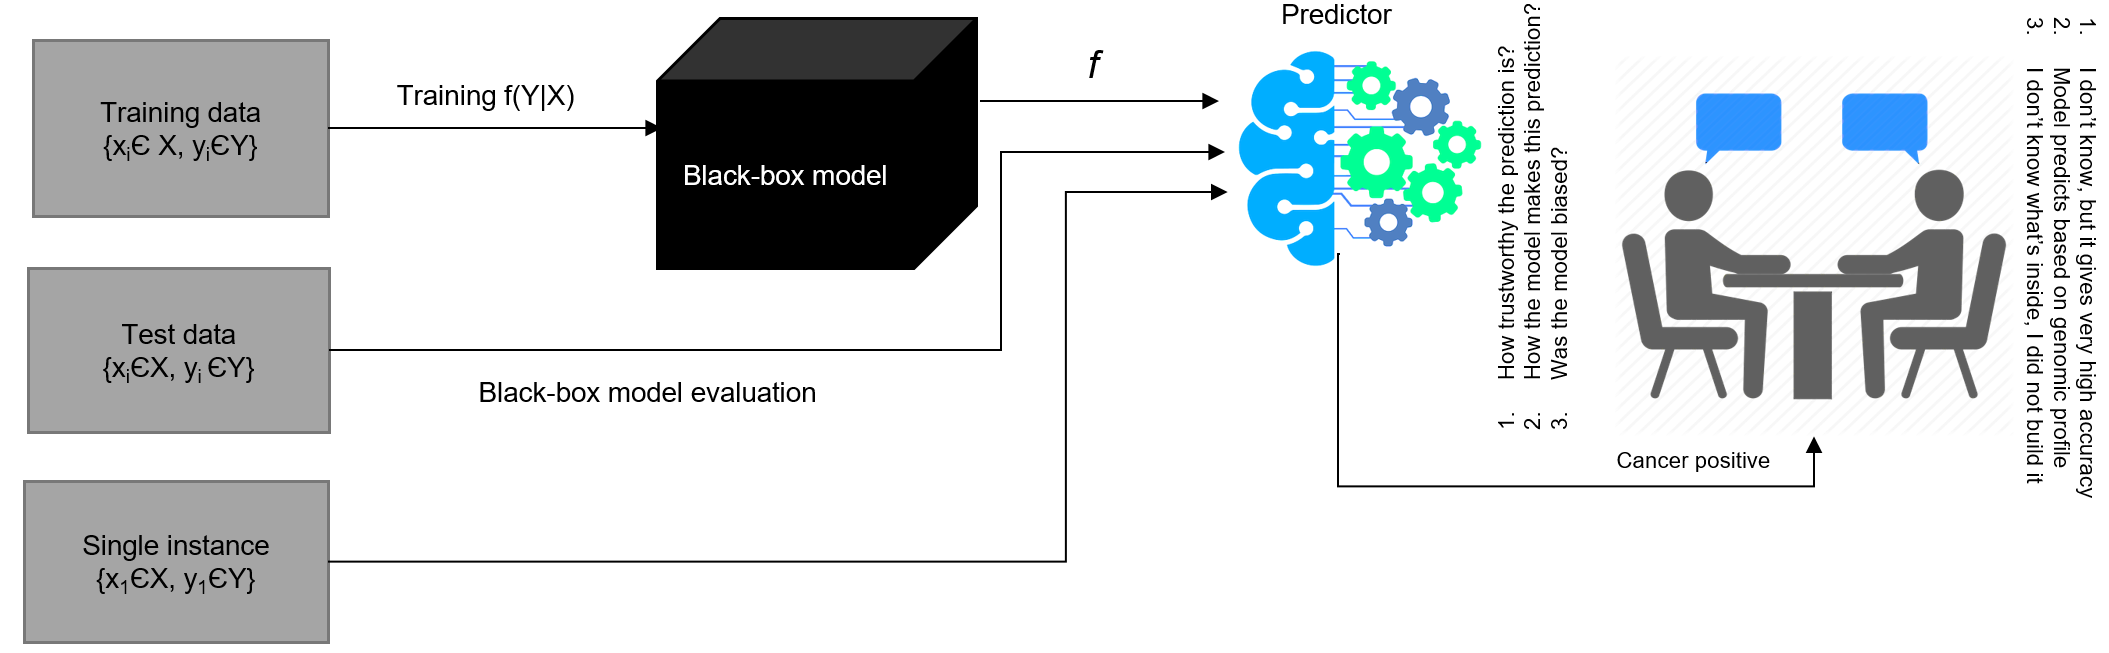
\includegraphics[width=0.9\linewidth]{images/bbm.png}
	\caption{Problems of model opacity}
    \label{fig:model_bbm}
    \vspace{-2mm}
\end{figure*}

\hspace*{3.5mm} Interpretable ML models allow healthcare experts to make reasonable and data-driven decisions to provide personalized diagnosis or treatment decisions that can lead to higher quality of service in healthcare~\cite{stiglic2020interpretability}. Based on this motivation, we model the prediction task as a multi-class classification problem. From a given genomic dataset $D$ about $n$ patients, $X$ = ${\mathbf{\{x_1,x_2,..., x_n}}\}$, where $x_k \in \mathbb{R}^{d}$. We consider classifying an individual $x_i$ into a specific cancer type based on his or her genomic profile. However, instead of classifying samples directly using their original representation $X$, we first transform the data with a nonlinear mapping $F_{\theta}: X \rightarrow Z$, where $\theta$ are learnable parameters and $Z \in \mathbb{R}^{K}$ is the learned or embedded feature space, where $K \ll D$.

\hspace*{3.5mm} To parametrize $F_{\theta}$, we employ neural network-based representation learning~(e.g., autoencoders) due to their function approximation properties and feature learning capabilities~\cite{xie2016unsupervised} from genomic data. Based on the embedding $Z$, classifier $F$ maps an input $x$ to an output $F: \mathbb{R}^{d} \mapsto y$. When we assume $F$ has a parametric form, we write $F_{\theta}$, where ${L}(F(x), y)$ denotes the loss function used to train $F$ on $D$ of input-output pairs $(x,y)$. However, since the decision made by the model cannot be traced back to the inputs, nor is it clear why the outputs are transformed the way they are. 

\section{Thesis Goal} \label{goals}
%Since an efficient ML model maybe better at predicting, detecting, and processing patterns then a human being, they intrinsically it cannot reason. Nevertheless, it is important to take fairness issues into consideration while developing such an explainable artificial intelligence~(XAI) system, 
Since many AI systems are being deployed to make important and life-changing decisions in sensitive environments~\cite{stiglic2020interpretability}, it is important to ensure that the decisions made by the system is not only accurate and trustworthy, but do not reflect discriminatory behavior toward certain groups or populations~\cite{mehrabi2019survey}. Thus, developing an explainable clinical decision support system~(XCDSS) system to improve the transparency and trustworthiness for real-life problems, e.g., to aid the cancer diagnosis. 

\begin{figure*}[h]
	\centering
	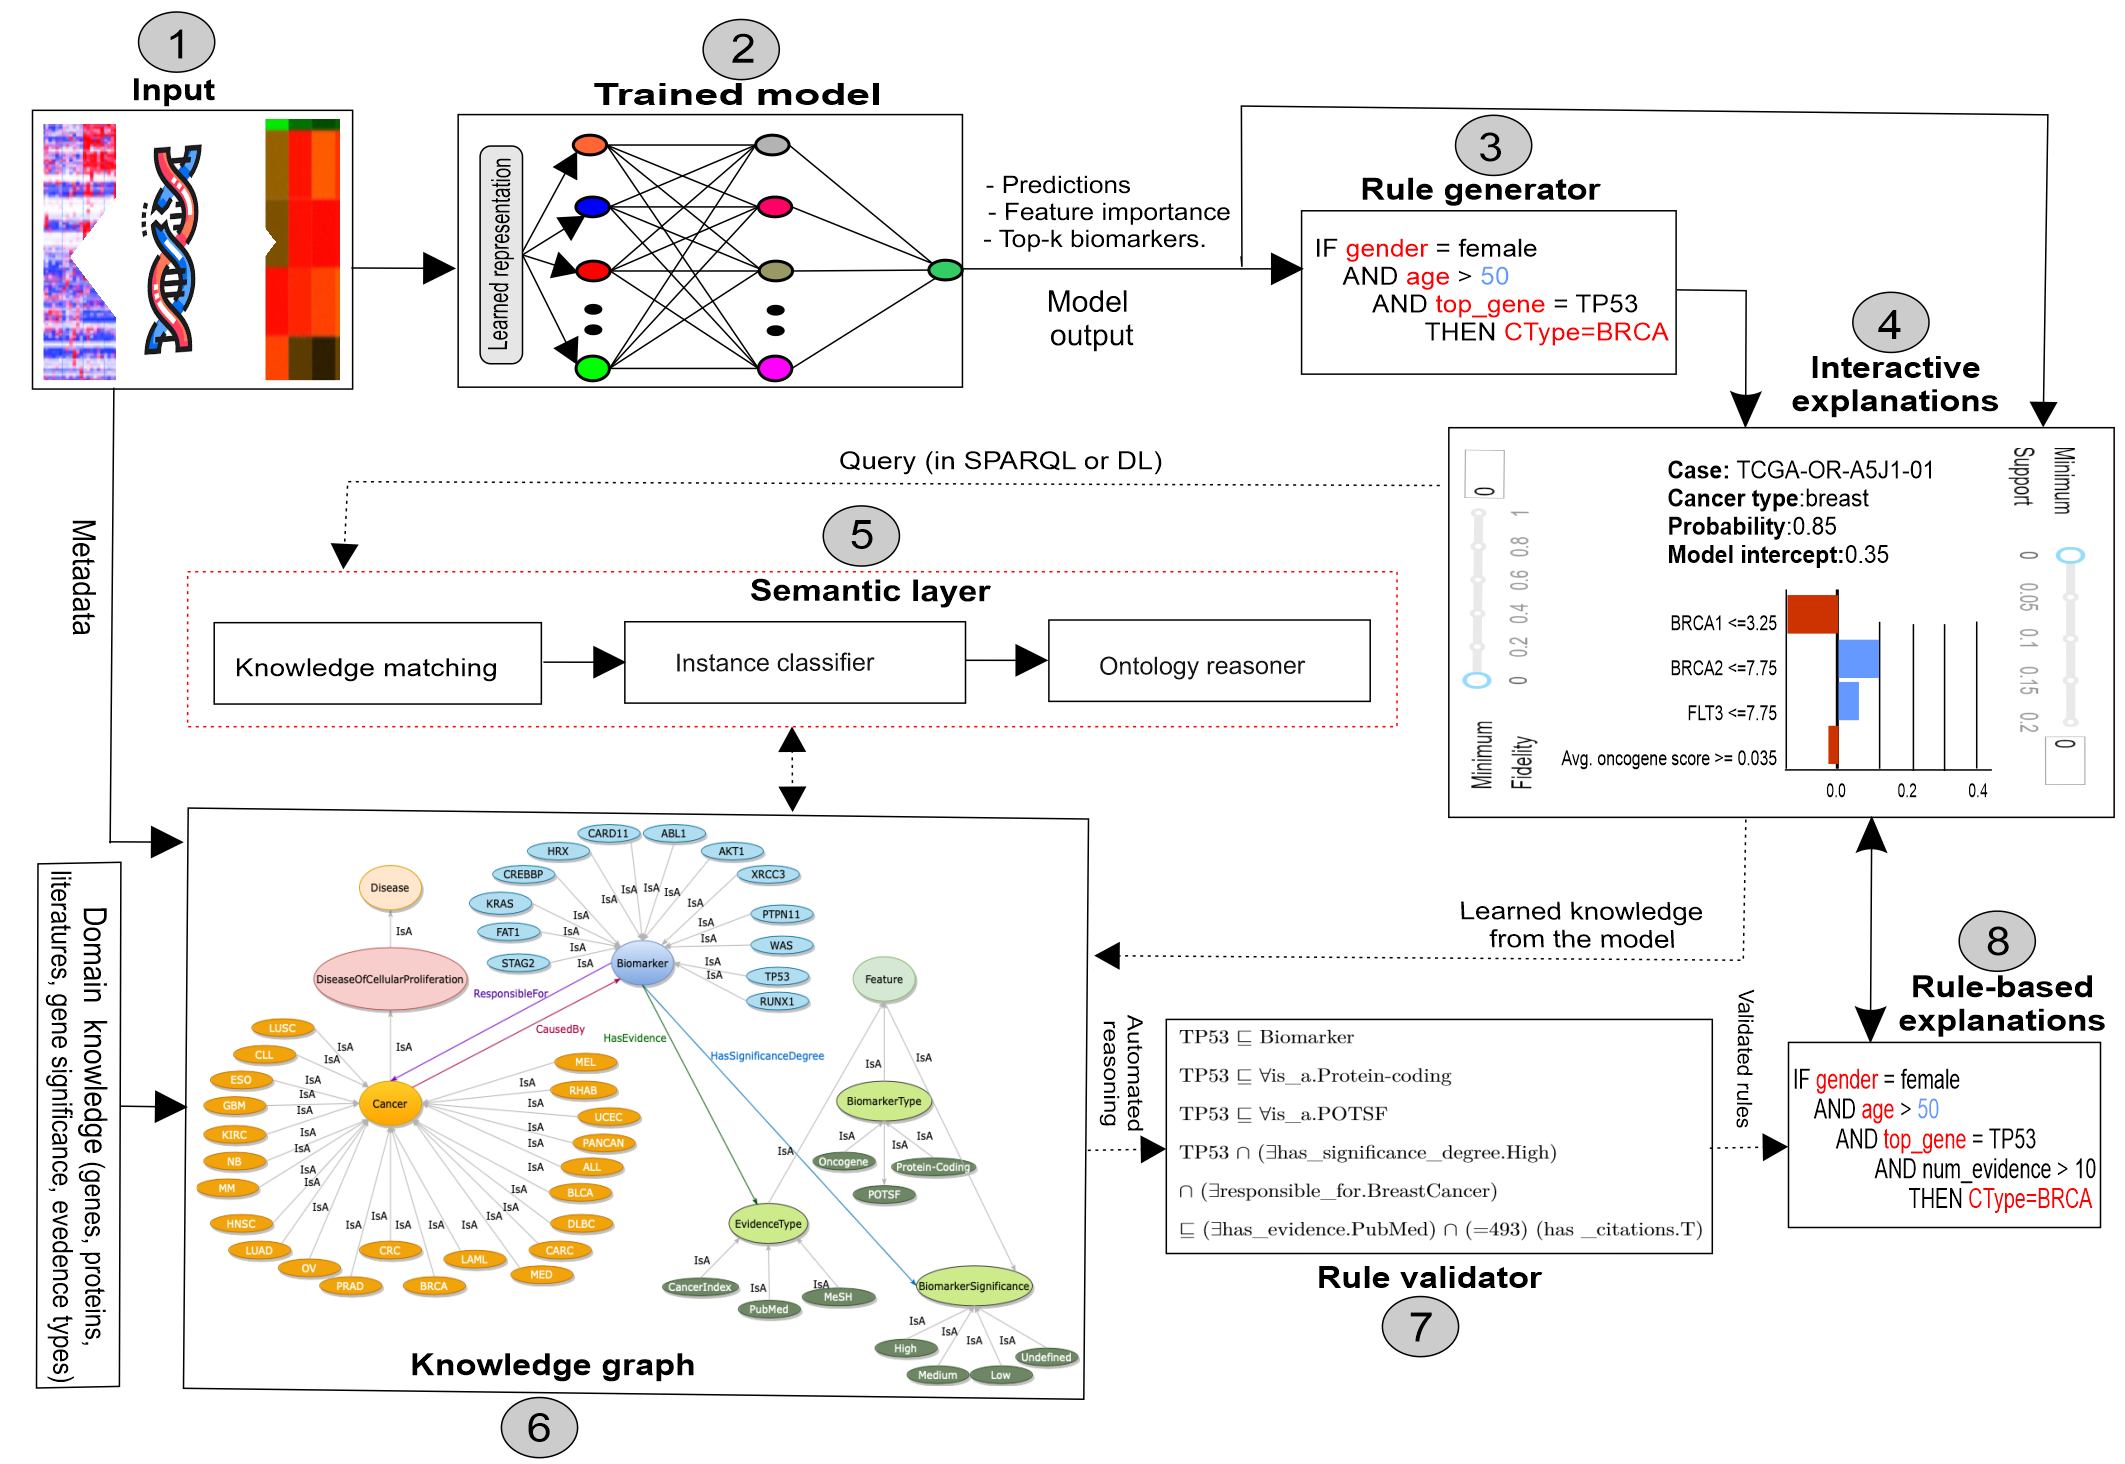
\includegraphics[width=\textwidth,height=95mm]{images/fair_rule_generator.png}	
    \caption{Workflow of the overall proposed approach}
	\label{fig:wf_overall_approach}
\end{figure*}

\hspace*{3.5mm} The proposed XAI model should be able generate accurate, fair, and trustworthy predictions in a transparent way, identifies misclassified instances, uses the existing knowledge from the knowledge base~(KB), and produces new knowledge, answers, and provides human-interpretable explanations about the prediction made. Making those predictions more accurately and explainable can: i) help doctors recommend better treatments, ii) help learn similarities between cancer types, iii) allow for drug repositioning, iv) and patients themselves can see what types of decision are made and why. 

\iffalse
\begin{figure*}[h]
	\centering
		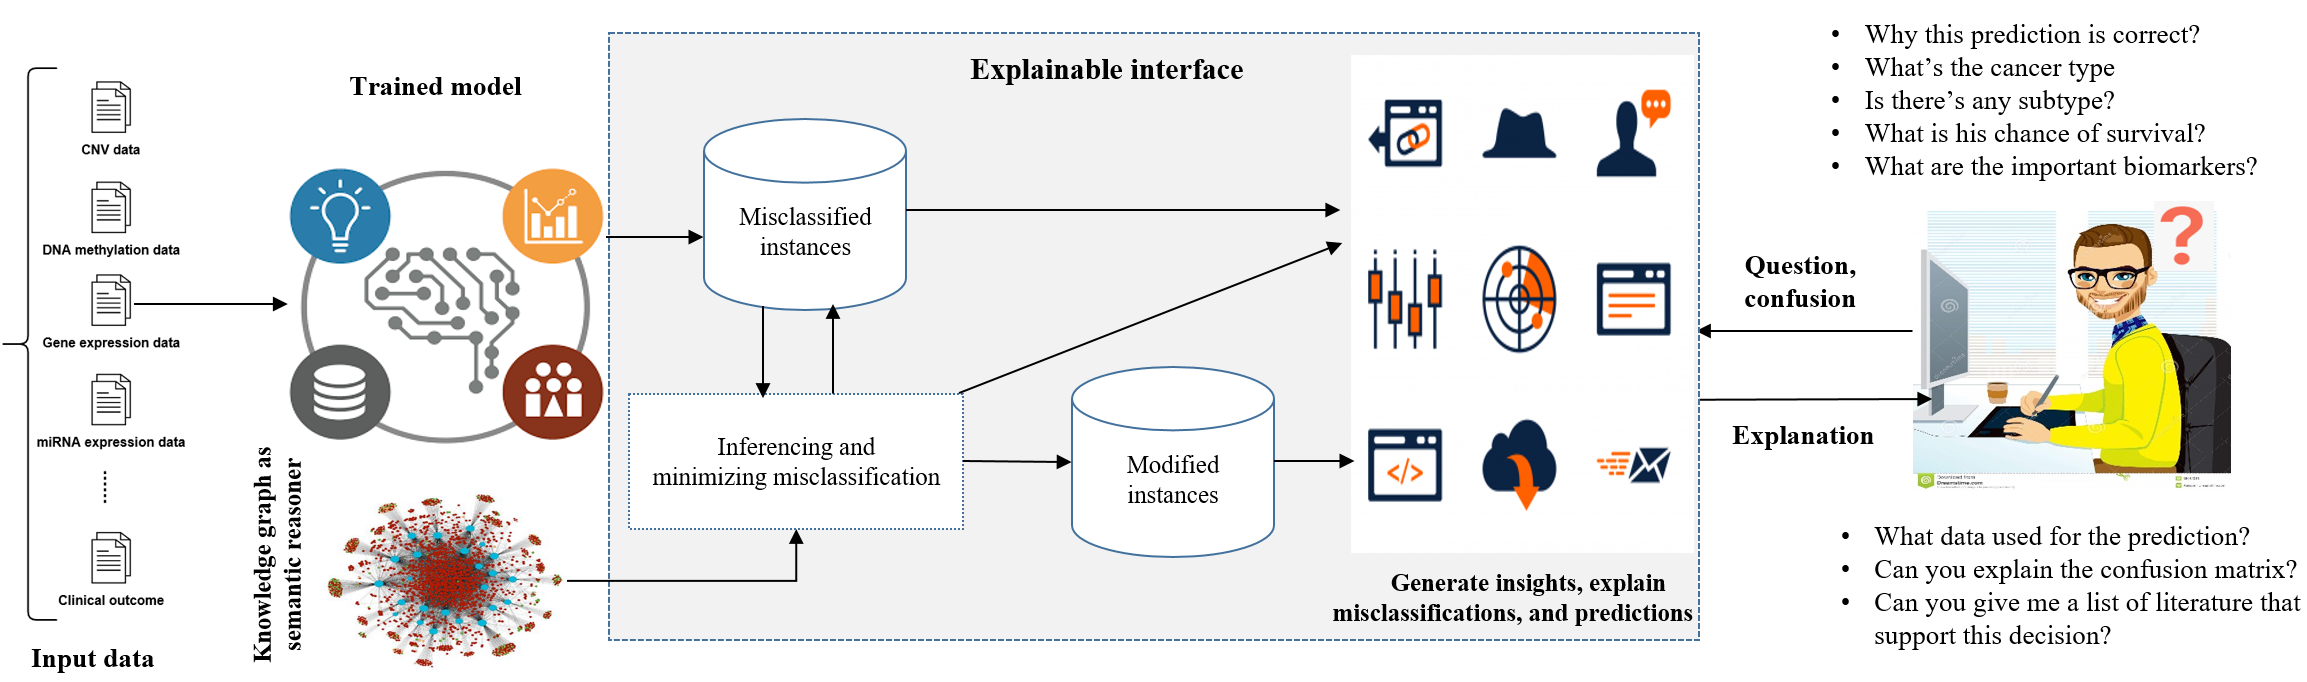
\includegraphics[width=\linewidth,height=60mm]{images/wf2.png}
		\caption{Workflow of the proposed model for explainable predictions of cancer}
        \label{fig:chapter_1_wf}
\end{figure*}
\fi 
%\subsection{Scope of the thesis}
%In the present study, a novel OA quantification solution based on multimodality integration is applied to overcome the limitations of the state-of-the-art approaches by effectively getting rid of the negative influences stemming from modality-forming principles. In terms of their complementary and application range, following a series of preprocessing methods, including contrast enhancement, noise elimination, and multi-slice integration, aiming at the same patient, radiographs and MRIs from axial, sagittal as well as coronal plane are respectively classified by their extracted features in the detected ROIs. Given supplying reliability and objectivity of the grading process, class-discriminating attention maps are generated by Class Activation Maps (CAM), prior to the averaging ensemble of models with the same modality and multimodality. 

\section{Hypotheses and Research Questions} \label{hypotheses}
To disseminating biological knowledge about carcinogenics through the proposed XAI system, the author suggests the following hypotheses to solve several research questions.  

\subsection{Research questions}
To develop an explainable model and to improve the fairness and transparency of a clinical decision support system~(CDSS), this thesis attempts to solve the following research questions: 

\vspace{-2mm}
\begin{itemize}[noitemsep]
    \item \textbf{RQ1}: How can multimodal data\footnote{e.g., genomics data such as GE, miRNA expression, copy numbers, and clinical outcome)} be more effective than unimodal data to provide accurate decision\footnote{e.g., how to accurately predict the outcome of a diagnosis decision?}? 
    \item \textbf{RQ2}: How to identify relevant features or factors\footnote{e.g., biomarkers for cancer diagnosis} that contributed most for a certain decision? 
    \item \textbf{RQ3}: How to provide human-understandable interpretations of predictions using fair decision rules? 
    %\textbf{${RQ}_5$}: How to generate human-interpretable decision rules to provide transparent cancer diagnosis? \\
    \item \textbf{RQ4}: How to disseminate and validate embedded domain knowledge\footnote{e.g., mechanisms of carcinogenesis}?
    \item \textbf{RQ5}: How to score a `black-box' model on fairness and transparency\footnote{e.g., why did the model behave in a certain way?}? 
\end{itemize}
\vspace{-2mm}

\subsection{Hypothesis}
We hypothesize that our approach based on DL and ML baselines with the explanation capability can be more effective at learning hierarchical features. We embed both local and global interpretability logic and interpretability layer to make ``black-box" model interpretable, which we hope to explain a data point $x$ using an explanation function $g$. We employ several local and global explanation methods to reason the predictions made by the model and mitigate the diagnosis decision biases. Local interpretability refers to an explanation giving reasoning why the model $F$ has predicted $F(x)$ for a fixed point $x$, during inferencing. Since providing human-level interpretability by ``zooming in" individual predictions makes the explanation more trustworthy~\cite{ribeiro2018anchors}, we answer the following questions based on local explanation methods: 

%\vspace{-2mm}
\begin{itemize}[noitemsep]
    \item Which feature $x \in X$ was most important for a certain prediction with $F$? 
    \item Which training data point $z \in \mathbb{R}^{K}$ was most important to $F(x)$? 
    \item What minimal change is necessary to input $x$ to change the output $F(x)$~(e.g., sensitivity analysis)? 
\end{itemize}
%\vspace{-2mm}

\hspace*{3.5mm} On the other hand, global interpretability signifies the overall transparency of the model inside a model on an abstract level. We answer following questions based on global explanation methods: 

%\vspace{-2mm}
\begin{itemize}[noitemsep]
    \item Which features in $X$ were most important across predictions for $F$? 
    \item Which training data points $z \in \mathbb{R}^{K}$ were most important to $F(X)$? 
    \item What minimal change is necessary to input $X$ to change the output $F(X)$~(e.g., sensitivity analysis)? 
\end{itemize}
%\vspace{-2mm}

\hspace*{3.5mm} We train and evaluate several deep architectures with interpretability capabilities, generate heat maps~(HM) for the classes and compute the feature importance in terms of mean absolute impact~(MAI) to identify important biomarkers, provide interpretations of the predictions, and decision visualization to make the cancer diagnosis transparent. Further, we validated our findings through functional analysis to make sure the selected genes are biologically trustworthy for the corresponding tumor types. Further, we will validate our findings based on the annotations provided by the TumorPortal to ensure the consistency and accuracy. In the same line, the symbolic reasoning over neural networks~(aka. neuro-symbolic reasoning), which can fuse the ability of DNNs models can be used to learn probabilistic correlations from scratch alongside abstract and higher-order concepts in order to provide human-interpretable explanations, and error corrections. \Cref{fig:wf_overall_approach} depicts the workflow of the proposed model for explainable predictions of cancer. This thesis make the following hypotheses, which will lead towards potential solutions to the research questions mentioned above in case they are confirmed:

%\vspace{-2mm}
\begin{itemize}[noitemsep]
    %\textbf{$H_2$}: neural representation learning can be more effective for learning high-level abstract features against data sparsity. \\
    \item \textbf{H1}: Multimodal genomics data and clinical outcomes can be used to train a multimodal neural network architecture to provide more accurate clinical diagnostic decision. 
    \item \textbf{H2}: A neural ensemble method, combining several deep architectures, can be more effective than structures solely based on a single model by reducing the generalization error. 
    \item \textbf{H3}: Since genomics data are high dimensional, embedding them into 2D raw images can help locate significant~(i.e, most and least) biomarkers. 
    \item \textbf{H4}: Interpretability provides insights on why/how a certain clinical diagnostic decision is recommended, highlighting significant~(i.e, most and least) biomarkers for further validation. 
    \item \textbf{H5}: Ontological reasoning can help characterize errors w.r.t their hierarchical relations from the KB that helps in decision reasoning.
    %A reasoner then can interact with the learning algorithm as a semantic referee. \\
    \item \textbf{H6}: Fair decision rules can be deduced by combining predictions and reasoning. 
\end{itemize}
%\vspace{-2mm}

\hspace*{3.5mm} To reach the goal, we solve the above research questions, which are driven by the hypotheses. \Cref{fig:wf_overall_approach} outlines the workflow of the overall approach. 

\section{Key Contributions} \label{contributions}
The main contributions of this thesis can be summarized as follows:

\begin{itemize}[noitemsep]
    \item We prepared a rich labelled multimodal genomics data for cancer type prediction that can be used to develop an efficient XCDSS\footnote{Explainable clinical decision support system}.  
    \item We trained several robust neural network models in which different interpretable~(e.g., feature attribution methods) and explainable logic~(e.g., Grad-CAM, LRP) are embedded. These approach enhance the capability of the learning algorithm to identify most significant biomarkers and provide class-specific explanations giving the top-k and common genes across cancer types. 
    \item We performed adversarial training to make the explainable model robust against different types of attacks, such as content moderation and out-of-distribution attacks. 
    \item A novel method of generating decision rules for cancer diagnosis by combing model prediction, biomarkers, and reasoning based on neuro-symbolic reasoning. 
    \item We took both proactive and reactive measures to make the diagnosis decision fair by mitigating different types of bias. 
    \item Comprehensive evaluations of our approach with detailed analyses of outcomes and comparisons with state-of-the-art. 
\end{itemize}

\hspace*{3.5mm} These contributions were reflected into 3 directions: i) peer-reviewed scientific publications, ii) public talks and presentations, iii) open source contributions~(i.e., implementations of some approaches presented). %A number of peer-reviewed publications were produced while conducting the work in this thesis. They are mentioned below, and a note is made to their relevant chapters. 

\subsection{Relevant publications}
The above contributions to science were reflected in a number of peer-reviewed publications. It is to be noted that some of the publications help build the foundations of this thesis. In addition, notes are made to their relevant chapters: 

\begin{enumerate}
	\item {Alokkumar Jha, Yasar Khan, Muntazir Mehdi, \textbf{Md. Rezaul Karim}, Qaiser Mehmood, Achille Zappa, Dietrich Rebholz-Schuhmann, and Ratnesh Sahay, ``Discovering Biomarker and Pathway for Gynecological Cancers", \emph{Journal of Biomedical Semantics}, 8(1), September 2017, DOI: 10.1186/s13326-017-0146-9.} 
	
	\textbf{Abstract}: In this paper, we present an approach to link and query different sequencing datasets such as TCGA, COSMIC, REACTOME, KEGG, and GO to indicate risks of different cancer types. We analyse the tissue expression of genes, CNV, somatic mutation, and promoter methylation to identify associated pathways and find novel biomarkers. 
	
	\textbf{Relevance}: this publication helps provide basic understanding of carcinogenics and different types of genomics data needed to be analyse towards biomarker discovery in \cref{chapter:introduction} and \cref{chapter:preli}.
	
	\textbf{Link}:~\url{https://jbiomedsem.biomedcentral.com/articles/10.1186/s13326-017-0146-9}
	
	\item \textbf{Md. Rezaul Karim}, Stefan Decker, Oya Beyan, ``Cancer Risk and Type Prediction Based on Copy NumberVariations with LSTM and Deep Belief Networks", \emph{Proc. of Artificial Intelligence International Conference (A2IC2018)}, November 21-23, Barcelona, Spain. 
	
	\textbf{Abstract}: In this paper, we apply DL methods to identify cancer and tumor types using CNVs extracted from cancer genomics data from TCGA. We identify and extract CNVs based on long short-term memory~(LSTM) and deep belief networks~(DBN). These were trained using two different representations of CNVs: based on oncogenes and all human genes. Due to lack of sufficient amount of labeled data, we pre-trained the DBN in an unsupervised way then the supervised fine-tuning was carried out using both feed-forward and LSTM networks. 
	
	\textbf{Relevance}: this publication was one of the first attempts to apply DL in cancer types prediction, which motivates us employing more advanced DNN architectures in chapter \ref{chapter:uni_modality}, \ref{chapter:multiodality}, \ref{chapter:xai}, and \ref{chapter:robustness}.
	
	\textbf{Link}:~\url{https://www.premc.org/doc/A2IC2018/A2IC2018_Book_Of_Abstracts.pdf}
	
	\textbf{GitHub}:~\url{https://github.com/rezacsedu/Cancer-Risk-Type-Prediction-CNV-LSTM-DBN}
	
	\item \textbf{Md. Rezaul Karim}, Oya Beyan, Achille Zappa, Ivan G. Costa, Dietrich Rebholz-Schuhmann, Michael Cochez, and Stefan Decker, ``Deep Learning-based Clustering Approaches for Bioinformatics", \emph{Briefings in Bioinformatics}, 02 February, 2020.
	
	\textbf{Abstract}: In this paper, we review state-of-the-art DL-based approaches for cluster analysis that are based on representation learning. We also discussed why and how the representation learning based on different autoencoder architectures are more effective at clustering high dimensional datasets than classic clustering algorithms~(e.g., K-means), covering bioimaging, GE, and biomedical texts. 
	
	\textbf{Relevance}: this publication forms the foundations of representation learning based on variational, LSTM, and convolutional autoencoders used in chapter \ref{chapter:multiodality}, \ref{chapter:xai}, and \ref{chapter:robustness}.

	\textbf{Link}:~\url{https://academic.oup.com/bib/advance-article/doi/10.1093/bib/bbz170/5721075}
	
	\textbf{GitHub}:~\url{https://github.com/rezacsedu/DL_Clustering_Bioinformatics}
	
	\item \textbf{Md. Rezaul Karim}, Michael Cochez, Oya Beyan, Dietrich-Rebholz Schuhmann, and Stefan Decker, ``Convolutional Embedded Networks for Population Scale Clustering and Bio-ancestry Inferencing", \emph{IEEE/ACM Transactions on Computational Biology and Bioinformatics}, 2020.
	
	\textbf{Abstract}: in this paper, we proposed convolutional embedded networks~(CEN) in which we combine two DNN architectures called convolutional embedded clustering~(CEC) and convolutional autoencoder~(CAE) classifier for clustering individuals and predicting geographic ethnicity, respectively, based on genetic variants~(GVs). We employed CAE-based representation learning on GVs from the `1000 genomes' and `Simons genome diversity' projects. This publication forms the foundations of representation learning based on CAE used in \cref{chapter:uni_modality} and \cref{chapter:xai}.

	\textbf{GitHub}:~\url{https://github.com/rezacsedu/Recurrent-Deep-Embedding-Networks}
	
	\item \textbf{Md. Rezaul Karim}, Stefan Decker, Oya Beyan, ``Drug-Drug Interaction Prediction Based on Knowledge Graph Embeddings and Convolutional-LSTM Network", \emph{In Proc. of ACM International Conference on Bioinformatics, Computational Biology, and Health-informatics~(ACM-BCB)}, Niagara Falls, New York, USA, September 7-10, 2019.
	
	\textbf{Abstract}: In this paper, we propose a new approach for predicting drug-drug interactions~(DDI) with Convolutional-LSTM network trained on multiple data sources. For this task we use drug features from DrugBank, PharmGKB, and KEGG drugs, which are integrated using Knowledge Graphs~(KGs). Our evaluations against several baseline models outperforms state-of-the-art approaches. 
	
	\textbf{Relevance}: this publication further motivates us employing Conv-LSTM network in \cref{chapter:uni_modality}.
	
	\textbf{Link}:~\url{https://dl.acm.org/doi/10.1145/3307339.3342161}

	\textbf{GitHub}:~\url{https://github.com/rezacsedu/DDI-prediction-KG-embeddings-Conv-LSTM}
	
	\item \textbf{Md. Rezaul Karim}, Ashiqur Rahman, Stefan Decker, and Oya Beyan, ``A snapshot neural ensemble method for cancer type prediction based on copy number variations", accepted for publication in \emph{Neural Computing and Applications}, 30 November 2019. 
	
	\textbf{Abstract}: in this paper, we used CNVs data covering different cancer types from The Cancer Genome Atlas~(TCGA).We construct two sparse representations of CNVs based on oncogenes and protein-coding genes. Then we train Conv-LSTM and convolutional autoencoder~(CAE) networks using both representations and create snapshots models. While the Conv-LSTM can capture locally and globally important features, CAE can utilize unsupervised pre-training to initialize the weights in the subsequent convolutional layers against the sparsity. Model averaging ensemble~(MAE) is then applied to combine the snapshot models in order to make a single prediction. 
	
	\textbf{Relevance}: this publication further forms the foundation of applying snapshot neural ensemble technique in chapters \ref{chapter:uni_modality} and \ref{chapter:xai}.
	
	\textbf{Link}:~\url{	https://link.springer.com/article/10.1007/s00521-019-04616-9}
	
	\textbf{GitHub}:~\url{https://github.com/rezacsedu/Cancer-type-prediction-CNV_LSTM-CAE} 
	
	\item \textbf{Md. Rezaul Karim}, Stefan Decker, Oya Beyan, ``Prognostically Relevant Subtypes and Survival Prediction for Breast Cancer Based on Multimodal Genomics Data", \emph{IEEE Access}, September 2019.
	
	\textbf{Abstract}: In this paper, we propose a new approach to analyze genomics data from TCGA to classify breast cancer patients based on their subtypes and survival rates. We used DNA methylation, GE, and miRNA expression data by creating a multiplatform network called multimodal autoencoders~(MAE) classifier to support each data type.
	
	\textbf{Relevance}: this publication further forms the foundation of applying MAE technique in \cref{chapter:xai}.
	
	\textbf{Link}:~\url{https://ieeexplore.ieee.org/document/8839793}
	
	\textbf{GitHub}:~\url{https://github.com/rezacsedu/MultimodalAE-BreastCancer}
	
	\item \textbf{Md. Rezaul Karim}, Michael Cochez, Oya Beyan, Stefan Decker, and Christoph Lange-Bever, ``OncoNetExplainer: Explainable Predictions of Cancer Types Based on Gene Expression Data", \emph{In proc. of IEEE International Concerence on Bioinformatics and Bioengineering~(BIBE 2019)}.
	
	\textbf{Abstract}: In this paper, we propose a new approach called \emph{OncoNetExplainer} to make explainable predictions of cancer types based on GE data on which we trained CNN and VGG16 networks using GradCAM++. We generate class-specific heat maps to identify significant biomarkers and computed feature importance to rank top genes across all the cancer types. Further, we identified top genes, and cancer-specific driver genes using gradient boosted trees and SHapley Additive exPlanations~(SHAP). Findings were validated with the annotations provided by the TumorPortal. 
	
	\textbf{Relevance}: this publication further forms the foundation of applying MAE technique in \cref{chapter:xai}.
	
	\textbf{Link}:~\url{https://ieeexplore.ieee.org/document/8941872}

	\textbf{GitHub}:~\url{https://github.com/rezacsedu/XAI_Cancer_Pred}
\end{enumerate}

%The articles in this dissertation are all related to knowledge evolution. The Venn diagram in fig. 7 depicts the relation between the research topics introduced in the previous chapter and the papers. Note that it does not necessarily depict the relations between the research topics in a broader sense1.  Each of the following sections describes the contributions to a topic from that figure. 

\subsection{Public conference talks}
The candidate participated several conferences as the part of the journey of this thesis: 
\begin{enumerate}[noitemsep]
    \item 10$^{th}$ International Semantic Web Applications \& Tools for Healthcare and Life Sciences~(SWAT4HCLS) Conference, Rome, Italy, 4-7 December, 2017 for providing a talk for the hackathon titled ``Deep Neural Networks for Analysing Cancer Genomics Data"\footnote{\url{http://www.swat4ls.org/wp-content/uploads/2017/11/Hackaton_SWAT4LS_DeepLearing_for_Cancer_Genomics.pdf}}
	\item 10th ACM International Conference on Bioinformatics and Computational Biology~(ACM-BCB), Niagara Falls, New York, USA, September 7-10, 2019 for presenting the paper titled ``Drug-Drug Interaction Prediction Based on Knowledge Graph Embeddings and Convolutional-LSTM Network".
	\item 1st Artificial Intelligence International Conference~(A2IC'2018), November 21-23, Barcelona, Spain for presenting the paper ``Cancer Risk and Type Prediction Based on CNVs with LSTM and DBN". 
	\item 19th IEEE International Conference on Bioinformatics and Bioengineering~(BIBE 2019), October 27-30, 2019, for presenting the paper titled ``OncoNetExplainer: Explainable Predictions of Cancer Types Based on Gene Expression Data".
\end{enumerate}

\subsection{Implementations}
All the codes in the preceding publications were written by the candidate. The candidate relied on existing libraries such as Keras, Sciket-learn, TensorFlow, PyTorch, DeepLearning4j, Apache Spark, and SHAP. All programs were implementation in Python. The software stack comprising Scikit-learn and Keras with the TensorFlow backend. Networks were trained on two computers: i) i7 CPU core, 32GB of RAM, Ubuntu 16.04 OS and Nvidia GTX 1050i GPU, ii) Intel(R) Xeon(R) CPU E5-2640, 256 of RAM, Ubuntu 16.04 OS. 
%In both machines, the CUDA and cuDNN enabled to make the overall pipeline faster. 

\hspace*{3.5mm} Besides semantic web technologies such as OWL, RDF, SPARQL, Jena, RDF4J, Fuseki, Virtuoso also utilized to some extent in certain publications. GitHub was extensively used for the  version control. 
Also, the Flask framework was used for wrapping up the explainable models and serving as an explainable interface. All the implementations were made open-source with a focus of reproduciblity. The GitHub page of the implementations can be found at \url{https://github.com/rezacsedu}.

\begin{figure*}[h]
	\centering
		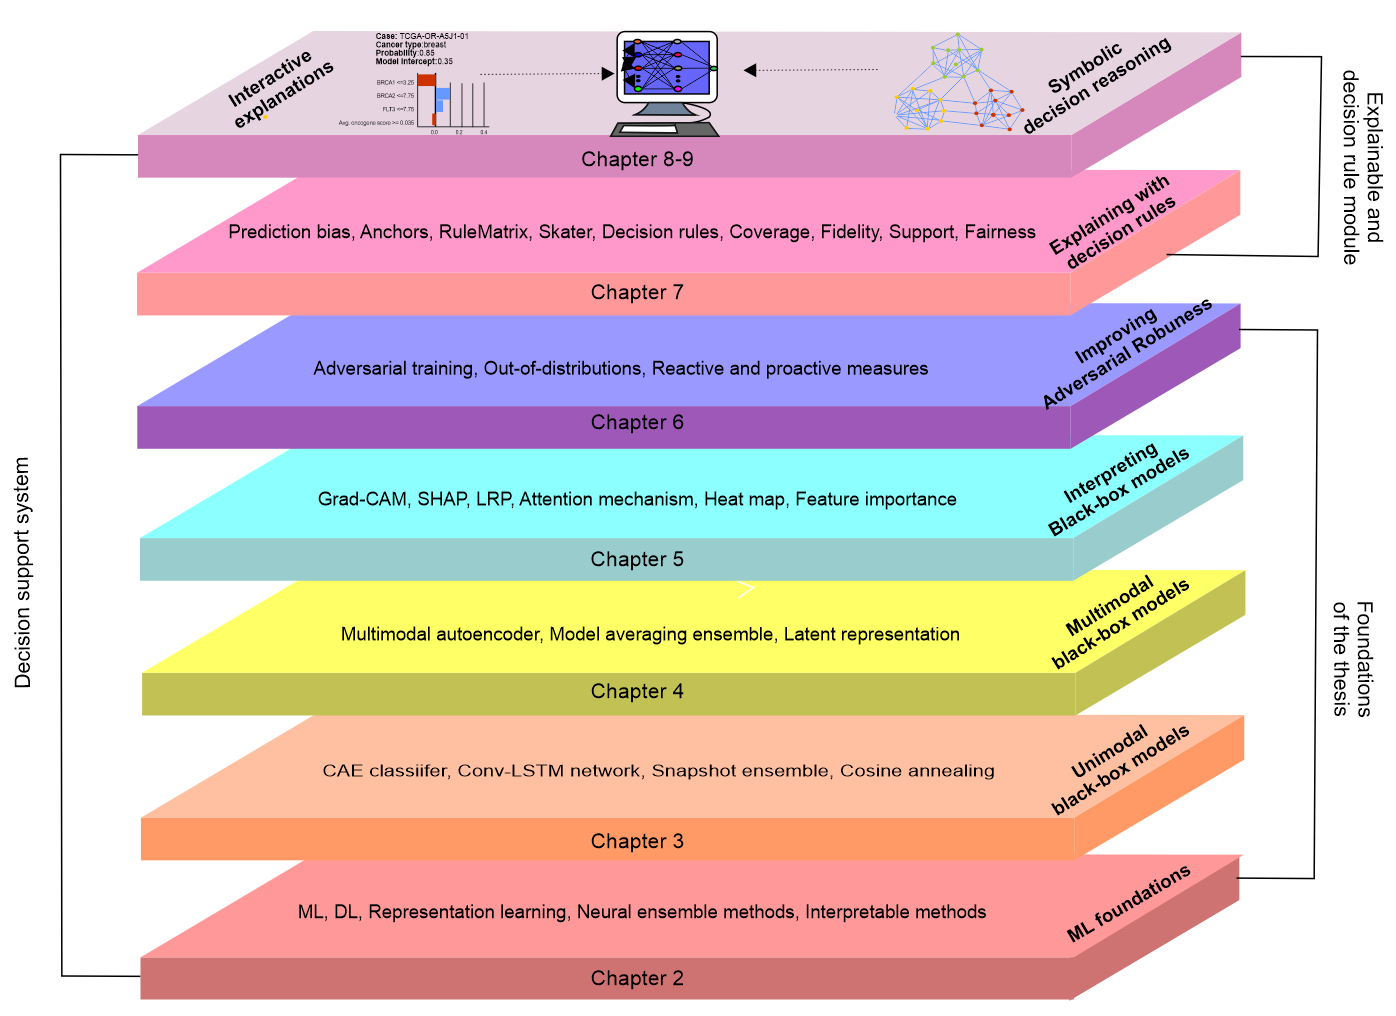
\includegraphics[width=0.7\linewidth,height=95mm]{images/chapter_outline.png}
		\caption{A bottom-up layout of the thesis, outlining the chapters}
        \label{fig:chapter_organization}
\end{figure*}

\section{Thesis Outline} \label{structure}
The rest of the thesis is structured into ten chapters. The brief overview of each chapter is as followed: \cref{chapter:preli} covers the foundations and concepts that will be used in the subsequent chapters. In \cref{chapter:uni_modality}, we develop predictive model based on single modality towards finding the association between CNV data and cancer, followed by the cancer type prediction task. In \cref{chapter:multiodality}, we extend the single modality based predictive model to multimodality-based cancer typing method by employing a multimodal neural network, but with a focus of breast cancer. In \cref{chapter:xai}, we employed two different approaches to open the `black box' uni/multimodal models towards making them explainable predictions of cancer types based on different genomics data. Besides, we identify significant biomarkers and computed feature importance in terms of mean absolute impact to rank top genes across all the cancer types. In \cref{chapter:robustness}, we apply different types of adversarial attacks on our models, including image content moderation, numeric data moderation, and out-of-distribution, followed by assessing the robustness against these scenario. 

\hspace*{3.5mm} In \cref{chapter:xai_rules}, we generate decision rules by combining model predictions and interpretations. Additionally, we identify  misclassified instances~(i.e., initial prediction by the model). In \cref{chapter:nsr}, we develop a  domain-specific ontology. Based on the biomarkers and their attributes, the reasoner tries to decide whether a biological entity is of correct types based on the ontological reasoning. The reasoner also help validate the findings and decision rules in order to deduce human-understandable decision rules in \cref{chapter:xai_rules}. In \cref{chapter:fairness}, we assess both explainability and fairness of our approach from statistical and philosophical perspective. \Cref{chapter:end} provides explanations and points out the relevance of the study, highlights its limitations and discusses future works before concluding the dissertation. 

